\documentclass{article}
\usepackage{cmap}
\usepackage[utf8]{inputenc}
\usepackage[english,ukrainian]{babel}
\usepackage{graphicx}
\usepackage{geometry}
\usepackage{listings}
\usepackage{float}
\usepackage{multicol}
\geometry{
	a4paper,
	left=20mm,
	right=20mm,
	top=20mm,
	bottom=20mm
}
\lstset{
	language=c,
	tabsize=4,
	keepspaces,
	showstringspaces=false,
	breaklines,
}
\graphicspath{ {./pictures} }
\setlength{\parindent}{4em}

\newcommand\subject{Алгоритми та структури даних}
\newcommand\lecturer{доцент кафедри ПЗ\\Коротєєва Т.О.}
\newcommand\teacher{асистент кафедри ПЗ\\Франко А.В.}
\newcommand\mygroup{ПЗ-22}
\newcommand\lab{12}
\newcommand\theme{Алгоритм пошуку Бойєра Мура}
\newcommand\purpose{Навчитися застосовувати алгоритм пошуку Бойєра Мура при розв’язуванні задач та перевірити його ефективність на різних масивах даних. Експериментально визначити складність алгоритму}

\begin{document}
	\begin{normalsize}
		\begin{titlepage}
			\thispagestyle{empty}
			\begin{center}
				\textbf{МІНІСТЕРСТВО ОСВІТИ І НАУКИ УКРАЇНИ\\
					НАЦІОНАЛЬНИЙ УНІВЕРСИТЕТ "ЛЬВІВСЬКА ПОЛІТЕХНІКА"}
			\end{center}
			\begin{flushright}
				Інститут \textbf{КНІТ}\\
				Кафедра \textbf{ПЗ}
			\end{flushright}
			\vspace{200pt}
			\begin{center}
				\textbf{ЗВІТ}\\
				\vspace{10pt}
				До лабораторної роботи № \lab\\
				\textbf{На тему}: “\textit{\theme}”\\
				\textbf{З дисципліни}: “\subject”
			\end{center}
			\vspace{112pt}
			\begin{flushright}
				
				\textbf{Лектор}:\\
				\lecturer\\
				\vspace{28pt}
				\textbf{Виконав}:\\
				
				студент групи \mygroup\\
				Коваленко Д.М.\\
				\vspace{28pt}
				\textbf{Прийняв}:\\
				
				\teacher\\
				
				\vspace{28pt}
				«\rule{1cm}{0.15mm}» \rule{1.5cm}{0.15mm} 2022 р.\\
				$\sum$ = \rule{1cm}{0.15mm}……………\\
				
			\end{flushright}
			\vspace{\fill}
			\begin{center}
				\textbf{Львів — 2022}
			\end{center}
		\end{titlepage}
		
		\begin{description}
			\item[Тема.] \theme.
			\item[Мета.] \purpose.
		\end{description}
		
		\section*{Лабораторне завдання}

	Розробити програму, яка:
		\begin{center}
3.       У файлі задано дві стрічки S та P. Довжина стрічок більша 0 і менша 10000, стрічки містять лише букви латинського алфавіту. Вивести номери символів в  порядку спадання починаючи з яких стрічка P входить в стрічку S.
		\end{center}
		
		\section*{Теоретичні відомості}
		Нажаль співпадіння зустрічаються значно рідше, ніж неспівпадіння. Тому виграш від використання алгоритму КМП в більшості випадків незначний. Інший алгоритму Бойера-Мура базується на наступній схемі: порівняння символів починається з кінця взірця, а не з початку. Нехай для кожного символу x взірця dx - відстань від самого правого у взірці входження х до кінця взірця. Припустимо, знайдено неспівпадіння між взірцем та текстом. Тоді взірець можна зразу посунути вправо на dx позицій що є більше або рівне 1. Якщо х у взірці взагалі не зустрічається, то посунути взірець можна зразу на всю його довжину m.
		
		В даному алгоритмі розглядається поняття стоп-символа - це є символ в тексті, який є першим неспівпадінням тексту і взірця при порівнянні справа (з кінця взірця). Розглянемо три можливих ситуації:
		
		1.  1.           Стоп-символ у взірці взагалі не зустрічається, тоді зсув дорівнює довжині взірця m.
		
		2.  2.           Крайня права позиція k входження стоп-символа у взірці є меншою від його позиції j у тексті. Тоді взірець можна зсунути вправо на k-j позицій так, щоб стоп-символ у взірці і тексті опинились один під одним.
		
		3.  3.           Крайня права позиція k входження стоп-символа у взірці є більшою від його позиції j у тексті. Тоді зсув дорівнює 1.
		
		\section*{Хід роботи}
		\begin{lstlisting}[language=C]
fn boyer_moore_search(
	pattern: &str,
	bm: BoyerMoore,
	text: &str,
	sleep_time: f32,
	stdout: &mut StandardStream,
	skip: bool,
) -> Result<(Vec<usize>, i32, i32)> {
	let mut occurrences = Vec::new();
	let mut alignments = 0;
	let mut comparisons = 0;
	
	let pattern = pattern.as_bytes();
	let text = text.as_bytes();
	let mut i = 0;
	
	while i < text.len() - pattern.len() + 1 {
		let mut shift = 1;
		let mut mismatched = false;
		let mut mismatch_index = 0;
		let mut skip_bc = 0;
		let mut skip_gs = 0;
		alignments += 1;
		
		for j in (0..pattern.len()).rev() {
			comparisons += 1;
			
			if pattern[j] != text[i + j] {
				skip_bc = bm.bad_char_rule(j, text[i + j] as char)?;
				skip_gs = bm.good_suffix_rule(j)?;
				shift = *[shift, skip_bc, skip_gs].iter().max().unwrap();
				mismatched = true;
				mismatch_index = j;
				break;
			}
		}
		
		if !mismatched {
			occurrences.push(i);
			skip_gs = bm.match_skip();
			shift = *[shift, skip_gs].iter().max().unwrap();
		}
		if !skip {
			visualize(
			stdout,
			from_utf8(text)?,
			from_utf8(pattern)?,
			i,
			mismatch_index,
			!mismatched,
			sleep_time,
			)?;
			println!("Comparisons: {}", comparisons);
			
			if i < text.len() - pattern.len() {
				if shift > 0 {
					println!("Shift: {}", shift);
				}
				
				print!("Press Enter to continue ...\r");
				io::stdout()
				.flush()
				.with_context(|| "Failed to flush stdout")?;
				let mut _input = String::new();
				io::stdin()
				.read_line(&mut _input)
				.with_context(|| "Failed to read input from stdin")?;
				print!("\u{1B}[F\u{1B}[K");
				io::stdout()
				.flush()
				.with_context(|| "Failed to flush stdout")?;
			}
			
			println!();
		}
		i += shift;
	}
	
	Ok((occurrences, alignments, comparisons))
}

		\end{lstlisting}
		
		\begin{figure}[H]
			\centering
			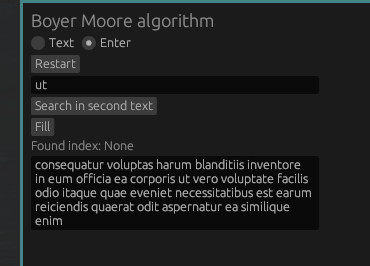
\includegraphics[scale=0.7]{1}
			\caption{Вигляд програми}
		\end{figure}
		
		\begin{figure}[H]
			\centering
			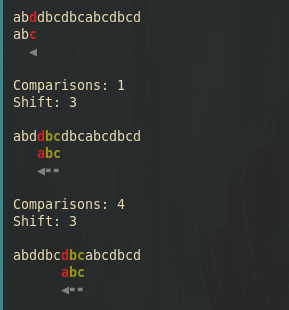
\includegraphics[scale=0.7]{2}
			\caption{Покроковий вивід}
		\end{figure}
		
		\section*{Висновоки}
		Під час виконання лабораторної роботи я навчився застосовувати алгоритм пошуку Бойєра Мура при розв’язуванні задач та перевірити його ефективність на різних масивах даних. Експериментально визначив складність алгоритму. 
		
	\end{normalsize}
\end{document}
